\section{Work Accomplished}\label{sec:work_accomplished}
In the previous section, the state of the art explored the various ways in which literature shows the integration of smart materials in actuator systems. Bistable elements using buckled beams shows a lot of promise due to the fact that they do not require energy to maintain the stable position and their potential energy can be used to trigger fast and dynamic strokes.

\subsection{Finite Element Modelling of SMA}\label{ssec:WA_FEM}
SMAs exist in various different stable phases which consists of the \emph{Martensitic (M)} phase and the \emph{Austenitic (A)} phase. The M phase can exist in either the \emph{Twinned M} phase or the \emph{Detwinned M} phase based on the stress experienced by the material. When the material reaches the Austenic transformation temperature ($\mathbf{A_s}$) threshold, the material will begin to transform from the M phase to the A phase i.e. the Austenitic transformation. Inversely, as the material cools down to the Martensitic transformation temperature ($\mathbf{M_s}$), it will begin to transform from the A phase to the M phase i.e. the Martensitic transformation. Since these transformations occur over a range in temperature, we must heat and cool well beyond the transformation temperatures. The SMA that in most likelihood will be used is a type of NiTiNOL variant with a relatively high transformation temperature (with $A_s$ around 50\degreeC) and thus exists primarily in the M phase at room temperature.

Since the stress distribution in a buckled beam is inhomogeneous, a Finite Element Modelling (FEM) simulation is more suited to handle the complexity of the calculations. The FEM simulation is performed using the Shape Memory Effect material property found in ANSYS Workbench. Using the nine parameters defined in the material property toolbox, we can simulate the shape memory effect. These parameters were obtained by consulting the material properties established in literature and datasheets from manufacturers\cite{divringi_advanced_2009}.

 So as to ascertain the reliability of the shape memory effect model created using ANSYS, a simple elongation test was performed. ANSYS workbench was used to model a simple SMA blade and a tractional strain of 8$\%$ was applied. The figure \ref{fig:FigElongationStressStrain}, shows the evolution of the internal stress of the SMA blade during the ANSYS scenario. This elongation test allows us to create a uniform stressed SMA blade that will perform the same phase changes as seen in the more complex buckled SMA beam.

\begin{figure}[H]
 \centering
 \begin{subfigure}[t]{0.45\textwidth}
    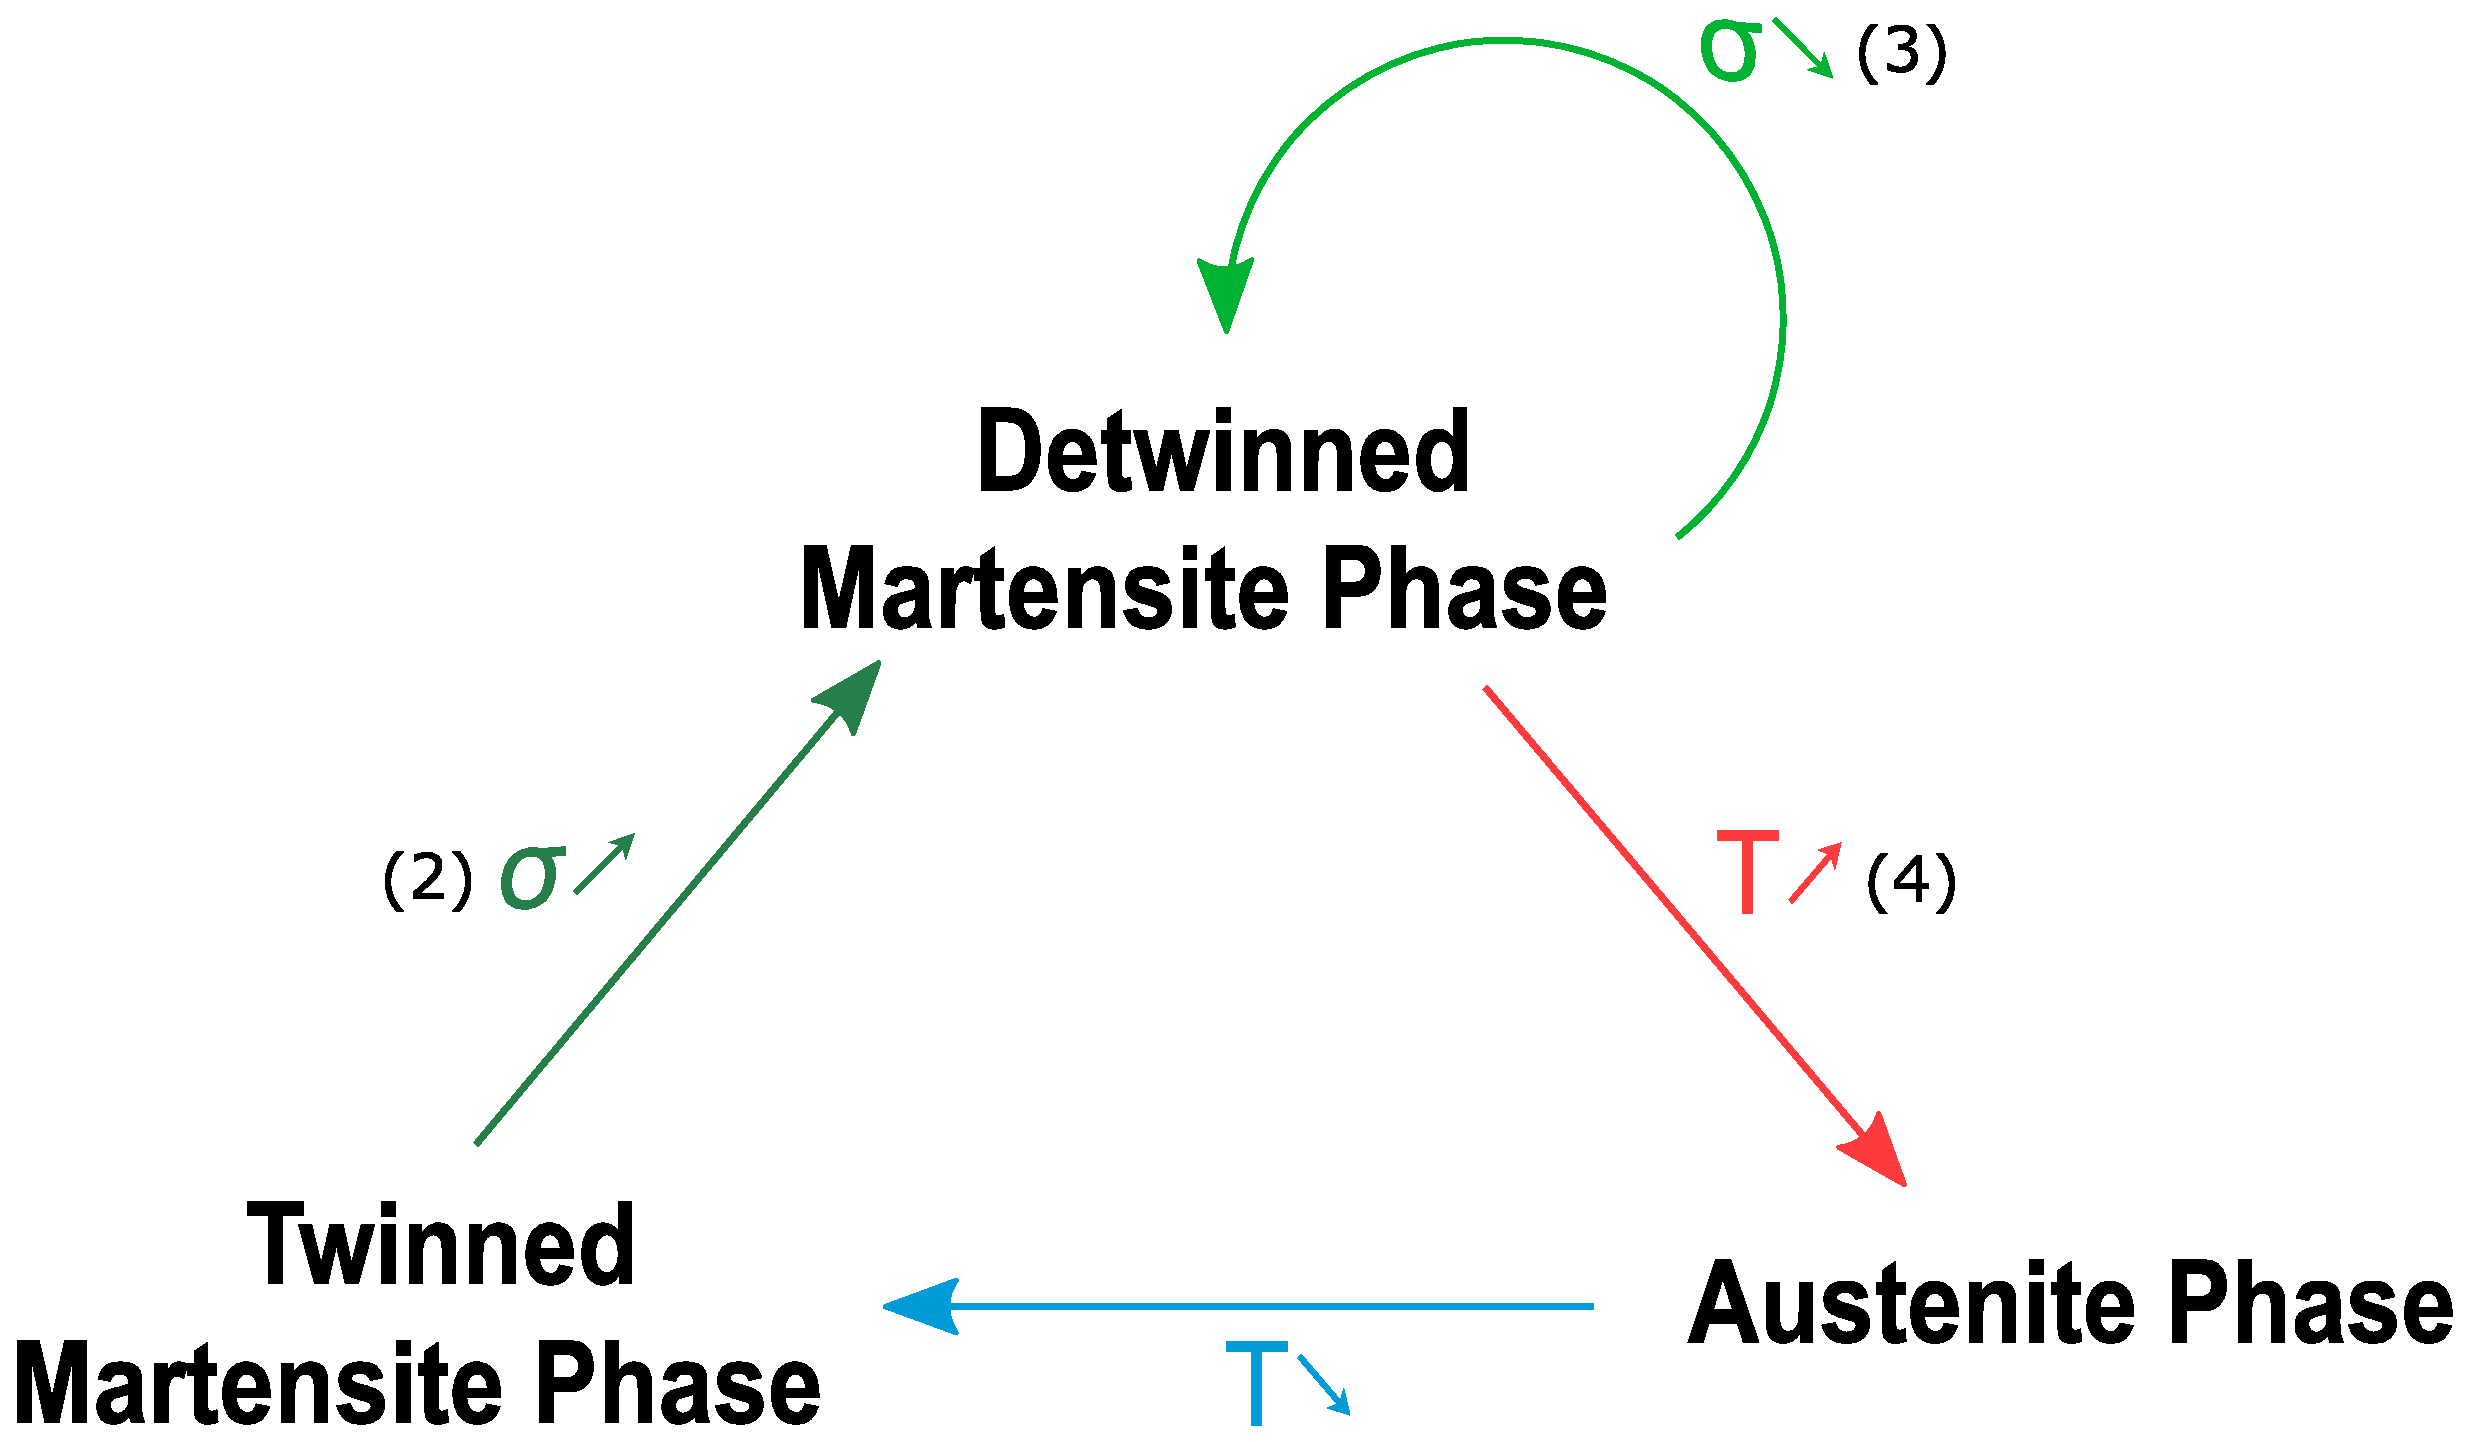
\includegraphics[width=\textwidth]{Figures/Phase_Transf_Diagram_Text.eps}
    \caption{Phase transformation diagram of a shape memory alloy. Here $\sigma$ represents the stress created by mechanical loading and T represents the temperature change due to thermal loading.}
    \label{fig:PhaseTransfDiagram}
 \end{subfigure}
	~
  %add desired spacing between images, e. g. ~, \quad, \qquad, \hfill etc.
   %(or a blank line to force the subfigure onto a new line)
 \begin{subfigure}[t]{0.45\textwidth}
    {\footnotesize
      \def\svgwidth{\textwidth}
      \input{Figures/FigElongationStressStrain.pdf_tex}
    }
    \vspace{-13pt}
    \caption{Finite element simulation of SMA Stress-Strain curve in traction and compression using a longitudinal bar}
    \label{fig:FigElongationStressStrain}
  \end{subfigure}
	\caption{The different phases and transformations of an SMA}
	\label{fig:SMAPhaseChange}
\end{figure}

The phase transformations can be seen in figure \ref{fig:PhaseTransfDiagram}. When a mechanical load is applied to the SMA while in its M phase, the material shears on an atomic level and this allows it to deform through a detwinning process at relatively low stress levels. This process allows the material to deform up to strains of 8$\%$. Strains larger than this will cause dislocations which are irreversible. In figure \ref{fig:FigElongationStressStrain}, we can see the various phase changes that occur within the SMA blade. Firstly, one end of the blade is fixed and the other end is subjected to a remote displacement so as to produce a strain. The resulting stress can be observed in region (1) of the figure. As the strain increases, the material reaches its stress threshold to transform from its twinned M phase to its detwinned M phase. This can be observed in region (2), where the strain increases rapidly. Once the blade has reached its maximal strain, the remote displacement is disabled. The region (3) shows that the blade loses its internal stress but remembers the deformation created by the mechanical load. Finally, the SMA blade is heated up and past its transformation temperature. This transforms the material from the A phase back to the M phase. This can be observed in region (4) where the graph shows the strain recovery of the material. This strain recovery is known as the Shape Memory Effect (SME). Thus, the strain of the material upon heating, immediately returns to zero and the elongation of the bar is recovered. This cycle can be observed in experimental tests studied in literature such as \cite{hongchun_xie_design_2007, liu_asymmetry_1998}

The FEM simulation was also used to ascertain the volumetric energy density of these SMA material. Here, again a simple monolithic beam was elongated and the work required for this elongation was estimated. Then, as the beam was heated above its transition temperature, the work output due to the strain recovery was measured. The difference between the two values allowed for the verification of the volumetric work presented by the literature shown in table \ref{tab:comparison}.

 % \begin{table}[H]
 % 	\centering
 % 	\footnotesize
 % 	\caption{SMA material property definitions}
 % 	\label{tab:matprop}
 % 	\begin{tabu} to 0.7\textwidth {X[l, 1.35] X[l, 0.65] X[r,3]}
 % 			\tableHeaderStyle{tableBlue}
 % 			\textbf{Property} & \textbf{Value} & \textbf{Definition} \\ [0.5ex]
 % 			$E_A$ [GPa] & 70 & Austenite Modulus \\
 % 			$E_M$ [GPa] & 30 & Martensite Modulus \\
 % 			$\nu$ & 0.3 & Poisson's Ratio \\
 % 			$H$ [GPa] & 1 & Hardening Parameter \\
 % 			$R$ [MPa] & 140 & Elastic Limit \\
 % 			$\beta$ [MPaK\textsuperscript{-1}] & 5.6 & Temperature Scaling Parameter \\
 % 			$T_0$ [K] & 323.15 & Reference Temperature \\
 % 			$\overline{\epsilon}_L$ [mm mm$^{-1}$] & 0.1 & Maximum Transformation Strain \\
 % 			$m$ & 0 & Lode Dependency Parameter \\
 % 	\end{tabu}
 % \end{table}

\subsection{Buckled beam modelling}
When a longitudinal monolithic beam is compressed and the critical axial load is reached, the beam will buckle and result in a bistable structure. The buckled beam will exist in two stable configurations as seen in the figure \ref{fig:States_Schema}. Specifically, this figure shows the two symmetrical stable states that the buckled beam can exist in for each given stable mode. The figure \ref{fig:Modes_Schema} shows the first three stable modes that are created when a longitudinal beam is pre-compressed.

\begin{figure}[H]
 \centering
 \begin{subfigure}[t]{0.45\textwidth}
   {\tiny
   \def\svgwidth{\textwidth}
   \input{Figures/BuckledBeamStable.pdf_tex}
   }
   \vspace{-10pt}
   \caption{Stable states of the buckled beam}
   \label{fig:States_Schema}
 \end{subfigure}
	~
  %add desired spacing between images, e. g. ~, \quad, \qquad, \hfill etc.
   %(or a blank line to force the subfigure onto a new line)
 \begin{subfigure}[t]{0.45\textwidth}
   {\tiny
   \def\svgwidth{\textwidth}
   \input{Figures/BuckledBeamModes.pdf_tex}
   }
   \vspace{-10pt}
   \caption{Diagram of the first three buckling modes}
   \label{fig:Modes_Schema}
  \end{subfigure}
	\caption{Representation of analytical model of buckled beam obtained from literature\cite{timoshenko_theory_1962}.}
	\label{fig:Buckled_Beam}
\end{figure}

When an axial load is applied to the longitudinal beam, the beam reaches a \emph{critical load} and is then deformed sideways, depending on the structure of the beam, to form one of the modes as seen in figure \ref{fig:Modes_Schema}.
% The modes can be described by the equation
% \begin{equation}
%   \label{eq:modeeq1}
%   \begin{split}
%     w = C\left(1-\cos\left(\frac{(j+1)\pi x}{l}\right)\right), \\
%     j = 1,3,5,...
%   \end{split}
% \end{equation}
% which describes the deflection for the odd modes where $C$ is an arbitrary constant, $l$ is the length of the beam and $x$ is the coordinate along the length of the beam. The equation
% \begin{equation}
%   \label{eq:modeeq2}
%   \begin{split}
%     w = C\Big[1-2\frac{x}{l}-\cos\left(k\frac{x}{l}\right) + \frac{2\sin(n_jx/l)}{n_j})\Big], \\
%     k = 2.86\pi, 4.92pi, 6.94\pi, 8.95\pi,...\quad j = 2,4,6,...
%   \end{split}
% \end{equation}
% describes the deflection of the even modes obtained from \cite{timoshenko_theory_1962}.
The figure \ref{fig:Modes_Schema} shows the two symmetric stables positions of the buckled beam. The beam can be triggered to switch from one of the states to the other by applying a vertical load at the apex of the curved beam. The displacement of the apex to a critical point will trigger the bifurcation or snap-through and thus the switching of states.

The modes seen in figure \ref{fig:Modes_Schema}, represent also the transition states of the beam as it transitions from one stable state to the opposing stable state \cite{rossiter_self-switching_2006}. When a vertical force is applied to the centre of the beam, the buckled beam is forced to transition to the third mode and then finally switches to the opposite state. While if a slight asymmetry is present in the fabrication of the beam or the actuation force, the beam transitions to the second state before switching to the opposite state.

Shape memory alloys can be used to create the buckled beam and can be used to supply the energy required to trigger the bifurcation. Since shape memory alloys can be activated using a thermal load, by applying a current through it, this allows the option to remove the central vertical force required and thus the external triggered required to trigger the switching. Thus, the SMA buckled beam actuation can be deemed a self-switching bistable mechanism. This paper will thus focus on the elimination of the external trigger in regards to standard bistable buckled beam actuators by using the potential energy stored within the SMA material.

\subsection{Self-switching of buckled SMA beam}
The next step of the research is to study the behaviour of a bistable buckled beam made entirely of an SMA. A monolithic beam of SMA is simulated and is then compressed from both ends to create the buckled beam as seen in figure \ref{fig:FigSMABlade}. The shape memory effect is only observed in areas of high stress where the material has exceeded the twinning threshold and has attained the twinned M phase as seen in figure \ref{fig:FigSMABlade}. Thus during the heating phase, these twinned M phase areas transform to the A phase and a vertical displacement of the apex of the buckled beam is observed. The goal of the research is to thus optimise the geometry so as to increase the maximum deformation of the buckled SMA beam when heated so as to create enough displacement that it will trigger bifurcation of the beam from one stable state to another. This behaviour can be deemed self-switching due to the fact that the system does not require an external trigger.

\begin{wrapfigure}{r}{0.45\textwidth}
	% \vspace{-5pt}
	\centering
  {\tiny
	\def\svgwidth{0.4\textwidth}
	\input{Figures/FigSMABlade3x_Edit.pdf_tex}
  }
	\caption{Simulated geometry of buckled SMA blade}
	\vspace{-10pt}
	\label{fig:FigSMABlade}
\end{wrapfigure}

The strain recovery of the buckled SMA beam can be optimised by increasing the percentage of material that has reached the twinned M phase. This requires the material to be stressed beyond its twinning threshold. The work initially strived to vary arbitrary parameters so as to observe an effect on the vertical displacement and thus, subsequently the beam's ability to self-actuate.

The simulations show that the optimization of the dimensions of the initial SMA blade alone cannot provide sufficient strain recovery to transition the buckled beam from one stable mode to another and that the parameters that influence the self-switching are difficult to pinpoint. On way this can be explained is due to the fact that the quantity of the material that transforms to the detwinned M phase due to the buckling is not sufficient to create enough vertical displacement so as to self-switch and due to the fact that the SMA is heated homogenously throughout the blade.

Thus another strategy is required to further improve the strain recovery observed in the buckled beam. Instead of varying the initial dimensions of the blade, the shape of the blade can be altered. Areas of increased thickness are added to the blade. In this case, the centre of the blade is thickened as seen in figure \ref{fig:modechange} so as to alter the behaviour.

In figure \ref{fig:modechange}, the stable mode after heating can also be observed. It shows that activation of the SMA creates a rotation of the centre vertex. The simulations concludes that by creating a blade with variable thickness, the behaviour of the system can be greatly affected. The thickened regions divide the beam into segments, allowing regions of the beam which are curved in the same direction to be actuated while regions that are curved in the opposite direction to not be actuated. This effect has been seen in literature\cite{rossiter_self-switching_2006} where the same principle is used for electrically stimulated self-switching buckled beams. The segmentation allows regions that will actuate in opposite directions to be reduced and thus further improve the vertical displacement.

\begin{figure}[H]
  \centering
  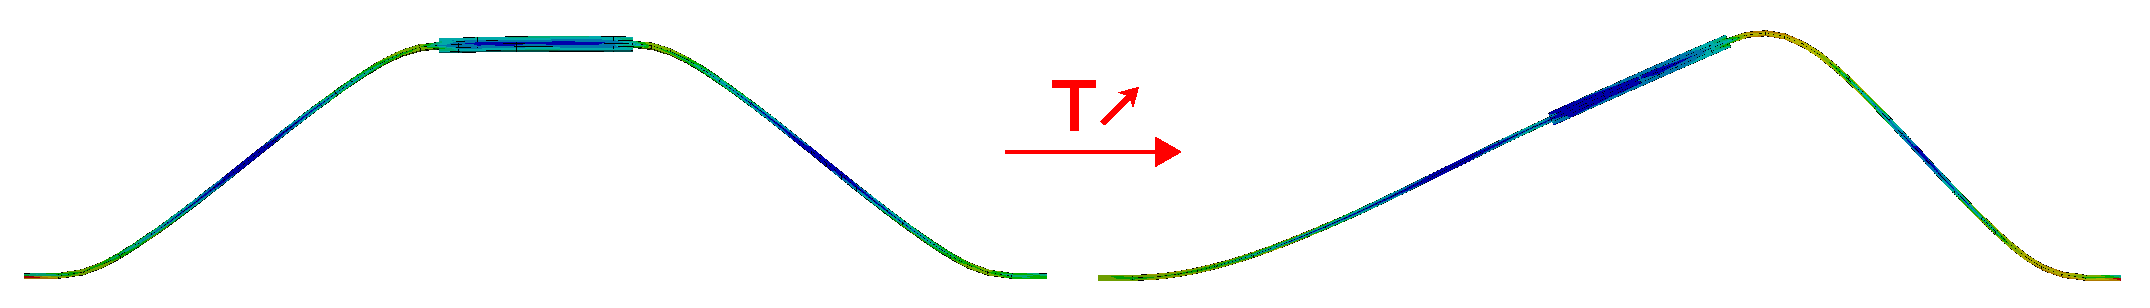
\includegraphics[width=\textwidth]{Figures/FigCentBumpTransformation.eps}
  \caption{Stable positions of the buckled beam before and after heating}
  \label{fig:modechange}
\end{figure}

% \begin{figure}[H]
%     \centering
%     \begin{subfigure}[t]{0.4\textwidth}
% 			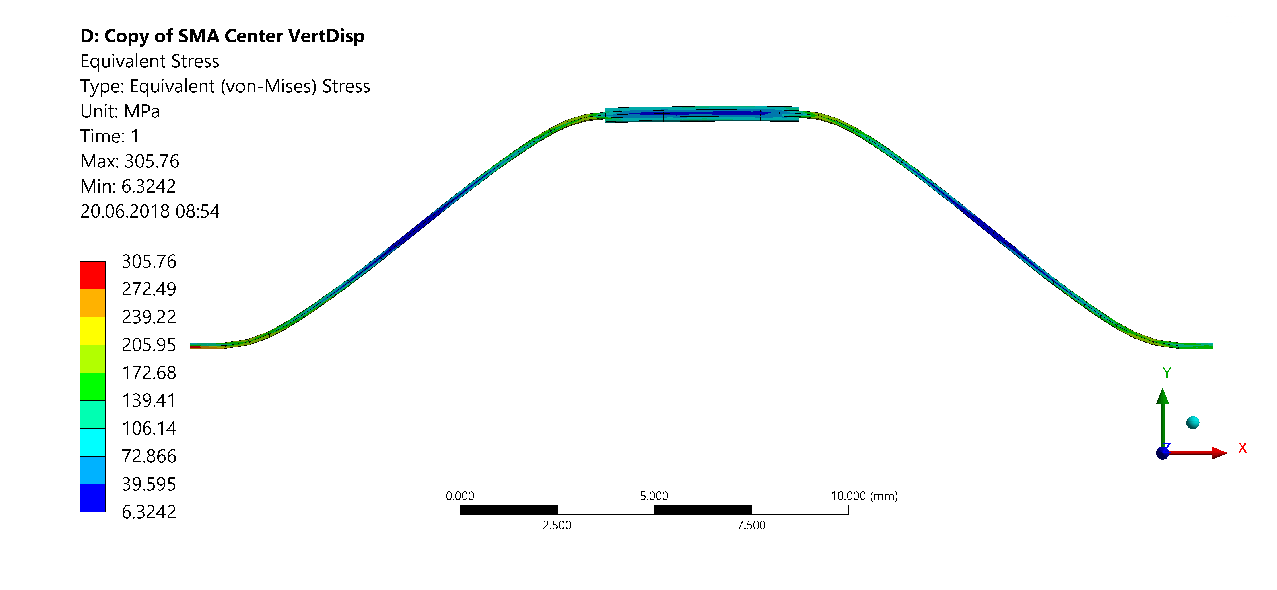
\includegraphics[width=\textwidth]{Figures/FigCentBumpBefore2x.eps}
% 			\caption{Before heating}
% 			\label{fig:modechangebefore}
%     \end{subfigure}
% 		~
%      %add desired spacing between images, e. g. ~, \quad, \qquad, \hfill etc.
%       %(or a blank line to force the subfigure onto a new line)
%     \begin{subfigure}[t]{0.4\textwidth}
% 			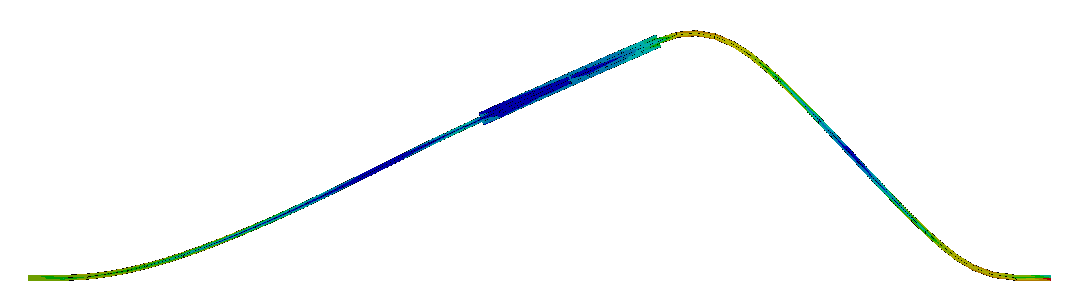
\includegraphics[width=\textwidth]{Figures/FigCentBumpAfter2x.eps}
% 			\caption{After heating}
% 			\label{fig:modechangeafter}
%     \end{subfigure}
% 		\caption{Stable positions of the buckled beam}
% 		\label{fig:modechange}
% \end{figure}

The direction in which the blade transitions is due to the convergence of the solution in the simulation. In an experimental scenario, the direction of the transformation can be controlled by creating an asymmetry in the thermal load or mechanical conditions. By applying a thermal load to either direction, the direction of the final stable mode can be chosen.

\subsection{Test bench layout}
So as to study the thermal properties of the SMA blade, a test bench that was designed to measure the time response of the SMA actuator is constructed as shown in figure~\ref{fig:test_bench}.
\newpage
% \begin{figure}[H]
%   \centering
%   \begin{subfigure}[b]{0.45\textwidth}
%     {\footnotesize
%     \def\svgwidth{\columnwidth}
%     \input{Figures/Test_Bench_Sample_Refactor.pdf_tex}
%     }
%     \caption{Layout of the test bench and examples of SMA blade samples generated using factors described in section \ref{ssec:WA_TRE}.}
%     % \vspace{-5pt}
%     \label{fig:test_bench}
%   \end{subfigure}
%   ~
%   %add desired spacing between images, e. g. ~, \quad, \qquad, \hfill etc.
%   %(or a blank line to force the subfigure onto a new line)
%   \begin{subfigure}[b]{0.45\textwidth}
%     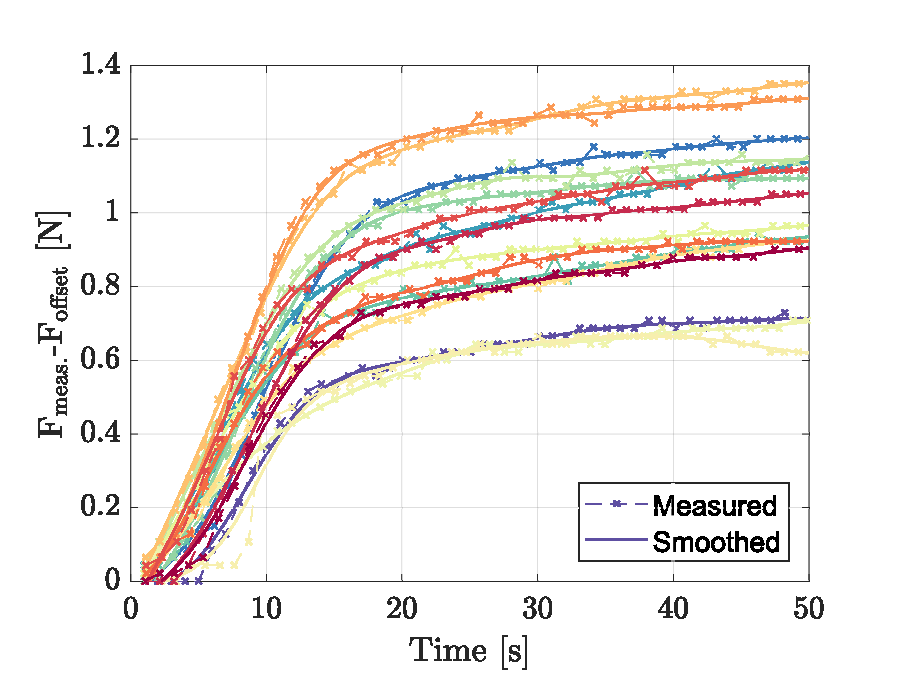
\includegraphics[width=\textwidth]{Figures/TB_Measurements.eps}
%     \caption{Force-time measurements obtained using the test bench.}
%     \label{fig:TB_Measurements}
%   \end{subfigure}
%   \caption{Representation of analytical model of buckled beam obtained from literature\cite{timoshenko_theory_1962}.}
%   \label{fig:Buckled_Beam}
% \end{figure}
\begin{wrapfigure}{r}{0.55\textwidth}
	\vspace{10pt}
	\centering
  {\footnotesize
  	\def\svgwidth{0.5\columnwidth}
  	\input{Figures/Test_Bench_Sample_Refactor.pdf_tex}
  }
	\caption{Layout of the test bench and examples of SMA blade samples generated using factors described in section \ref{ssec:WA_TRE}.}
	\vspace{-5pt}
	\label{fig:test_bench}
\end{wrapfigure}

An SMA blade is fixed between two electrodes which allow an electrical current to flow through the system. In this setup, the right electrode is part of the main body of the test bench while the left electrode is placed on a linear guide in order for it to be able to move only unidirectionally. Using this mobile part, the blade is preconstrained while in its M phase i.e. at low temperature. A force sensor is then placed behind the left electrode and fixed to the bench to measure the force applied by the SMA actuator while it tries to return to its initial shape during the transition from the M phase to the A phase, i.e. heating. The time required for the blade to reach its maximum force output can then be measured.

\subsection{Thermal response enhancement}\label{ssec:WA_TRE}
% \begin{wrapfigure}{l}{0.45\textwidth}
% 	\vspace{-10pt}
%     \centering
%     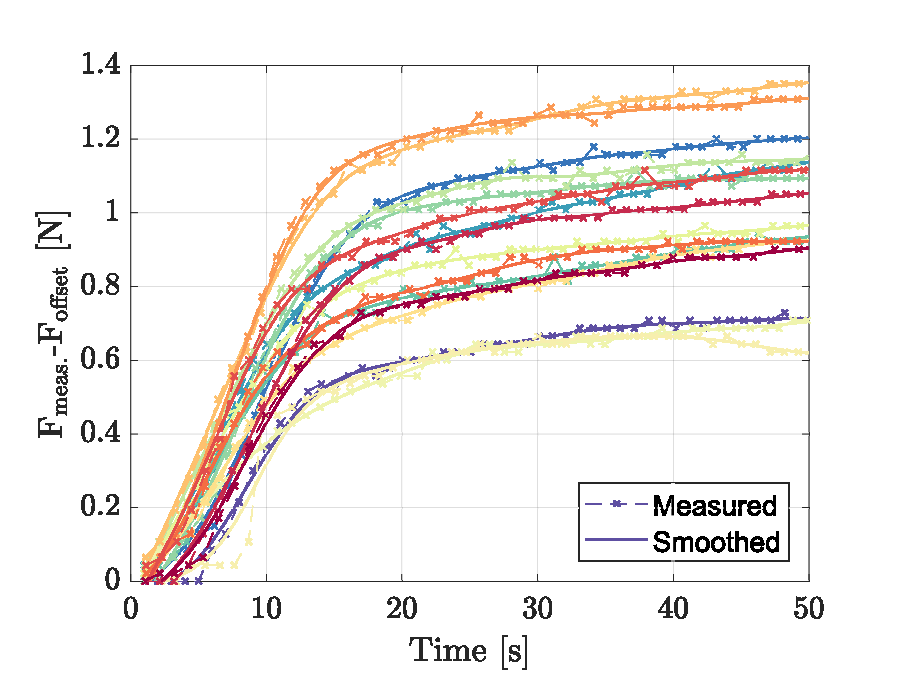
\includegraphics[width=0.45\textwidth]{Figures/TB_Measurements.eps}
%     \vspace{-20pt}
%     \caption{Force-time measurements of the d ifferent SMA blades obtained using the test bench.}
% 		\vspace{-10pt}
%     \label{fig:bar1}
% \end{wrapfigure}

This next section aims to optimise the heating of the SMA in critical sections and thus improve the force output and actuation times of the SMA actuator. The SMA blades are actuated using Joule heating where a current is passed through the blade and the internal resistance is used to heat the blade. Thus, the geometry of the blade is critical when optimizing the time response of the shape memory effect. The design of the SMA blades were created based on the location and orientation of perforations that were placed on the surface of the blade. The volume of material of the blade was also kept constant so as to have the same quantity of material to be heated during each run. This is controlled by ensuring that the thickness of blades are the same and that the total surface area is constant between each blade.

\begin{figure}[H]
  \centering
  \begin{minipage}{.45\textwidth}
    \centering
    \vspace{-10pt}
    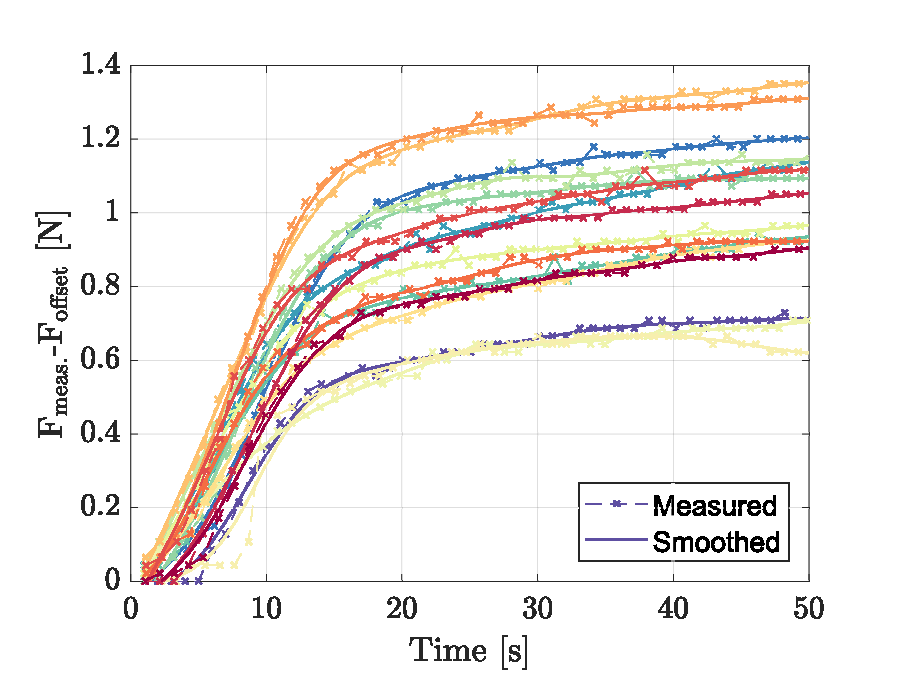
\includegraphics[width=\textwidth]{Figures/TB_Measurements.eps}
    \vspace{-20pt}
    \caption{Force-time measurements of the different SMA blades obtained using the test bench.}
		\vspace{-10pt}
    \label{fig:TB_Measurements}
  \end{minipage}%
  \hfill
  \begin{minipage}{.47\textwidth}
    \centering
    \vspace{-6pt}
    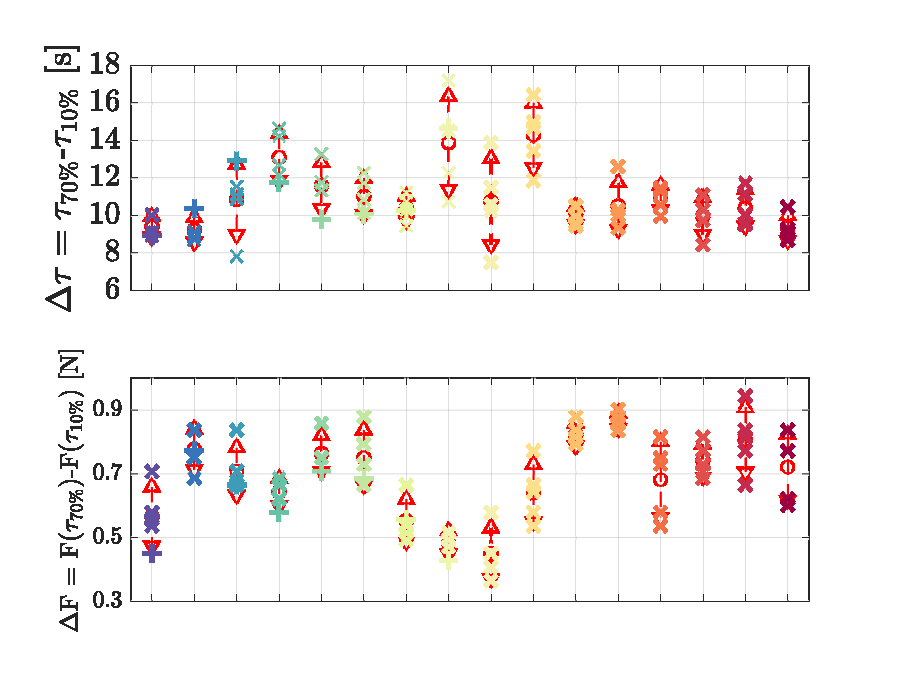
\includegraphics[width=\textwidth]{Figures/Had_RawData.eps}
    \vspace{-26pt}
    \caption{Results of the experiment conducted on the different SMA blade shapes showing the effect on the force output and the time constant.}
    \vspace{-10pt}
     \label{fig:Had_RawData}
  \end{minipage}
\end{figure}


% The design of the SMA blades was created based on four factors as defined below while also keeping the volume of material used constant:
% \begin{enumerate}[label=\textbf{~~~~Factor $x_{\arabic*}$}:,align=left]
%   \item Number of perforations along the width
%   \item Position of the holes along the length
%   \item Number of perforations along the length
%   \item Orientation of the perforation
% \end{enumerate}
The conventional option for the design of the test would be to design changes in the beam based on one factor at a time and observe the effect on the time response. This method is inefficient and time-consuming. Furthermore, the material is quite expensive, so extracting quality information for multiple construction factors from each blade is primordial. Thus, the effect of each parameter has been explored using a statistical approach based on a Hadamard matrix as presented in the work \ref{bib:TimeResponse}. This experiment performs an analysis of the factors with respect to the time response in terms of the force-time derivative while reducing the number of runs and the quantity of material used.

% \begin{wrapfigure}{r}{0.46\textwidth}
%    \vspace{-10pt}
%     \centering
%     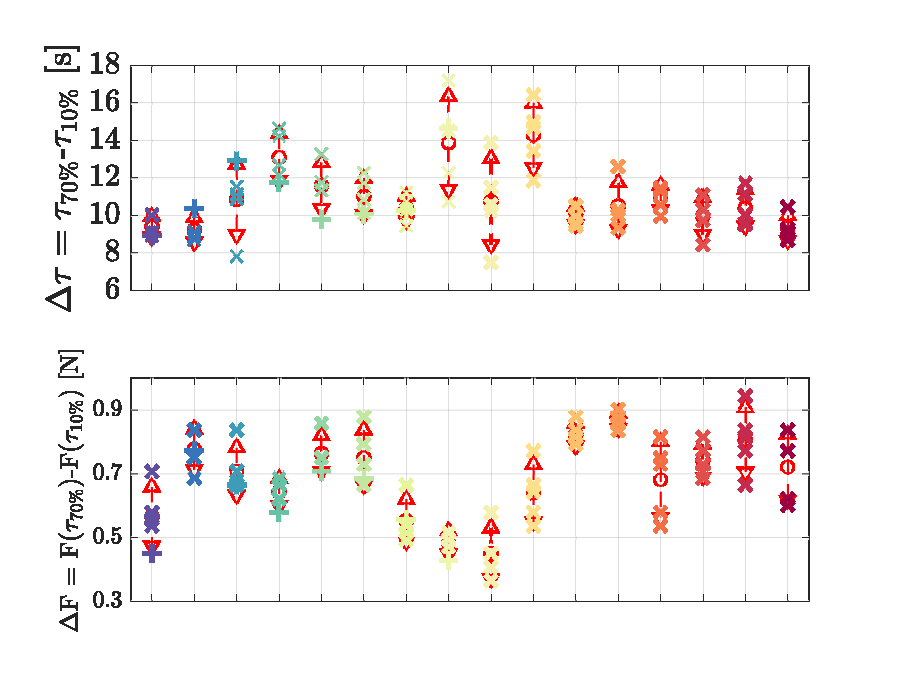
\includegraphics[width=0.5\textwidth]{Figures/Had_RawData.eps}
%     \vspace{-25pt}
%     \caption{Results of the experiment conducted on the different SMA blade shapes showing the effect on the force output and the time constant.}
% 		\vspace{-10pt}
%     \label{fig:bar1}
% \end{wrapfigure}

Here, the material used was a NiTiNOL with a low transformation temperature and thus existed mostly in the A phase at room temperature. Thus, due to a combination of ineffective power management during the heating process and the refrigeration required to observe the SME in the blade, the time response of the blades are much larger than the required use case scenario. Nevertheless, the experiment shows that the test bench can be used to create a preliminary test with the ability to measure the time response of a heated buckled SMA beam. The experiment was also able to shows that for the same quantity of material and by just changing the location of the perforations on the blade, the time responses can be improved.
% A linear fit of the force derivative with respect to time $\frac{dF}{dt}$ was performed, in the form of $\frac{dF}{dt} \sim x_1+x_2+x_3+x_4 $ (in Wilkinson notation) for the Hadamard with one run, five runs, and the full fold-over. The upper plot of figure \ref{fig:bar1} represents the influence of each factor upon the experiment with respect to the residual of this model. It is desirable to obtain coefficients whose significance is high with F-value $\geq$ 1. The lower plot represents the p-value, which is the probability of having validated a hypothesis by chance. In this case, the hypothesis is that factors have a non-zero influence in the model; meaning that small p-values (being sure that the parameters have a non-null influence) are desirable. It was deemed that concluding results should have p-values $\leq$ 0.05. Given their corresponding p-values, it could be affirmed that the factors $x_2$, $x_3$ and $x_4$ indeed affect the force vs time of the SMA blade; the longitudinal centring of the perforations, the number of them and their orientation, respectively.

The work \ref{bib:TimeResponse} shows that the effective use of power in the SMA blade can lead to better output forces and better time responses. The response of a SMA blade in terms of maximal force-time derivative can be optimised by carefully placed perforations. Indeed, an improvement by a factor of 3 could be observed between the highest and the lowest response in this experiment using the same quantity of material. This technique could be used in combination with the buckled SMA beam to efficiently heat the appropriate regions of the blade and eventually create a self-switching SMA actuator. The perforations create zones of higher resistance and thus more effective heating. This same principle can be used to find the appropriate areas to place printed coil heaters to further optimize the time response of the SMA actuator.
